\section{Progress to Date}
\label{sec:progress}

\subsection{Overview}
The project is on track to meet the targets set in the specification. The first one is the implementation of the web app and the scenario generation by the due date of the progress report. The web app has almost all features required for simulating an exam scenario functioning, with the last features being voice input and the ability to connect to the R/T web server. The R/T web server, has its structure planned out and is missing only a subset of the R/T parsing methods yet to be implemented.

\subsection{The Web App}
The first half of the first term has been predominantly focused on developing the web app described in objective 2 which will form the user interface (UI) of the system. As mentioned in the specification resources, the web app uses SvelteKit, which provides both the HTML component language Svelte and a router system for handling endpoint requests.

\subsubsection{Design Choices}
Reflecting the set of equipment and resources available in the exam, the interface has been designed to be minimal and simple. All elements are centred in the web page, with the most important at the top, in such a way that on a 1080p screen in all three target browsers (Chrome, Safari and Firefox) all elements required for a scenario are shown without the need to scroll.

The virtual radio and transponder are Svelte components, themselves comprising other smaller Svelte components which share properties and styles, in such a way that when a sub component's property changes the value bubbles up to the parent component. This allows complex behaviour such as changing the mode of a dial sub component being registered by its parent component, allowing the system to check if the radio has been set to the correct mode for the scenario state just by checking the radio component's properties. All components are written in just HTML, CSS and JavaScript, which has allowed the use of code libraries, reducing the amount of new code needed to create the interface. Despite this, the dials and displays were written from scratch as no similar components were found that met the requirements of the web app.

\begin{figure}[H]
    \centering
	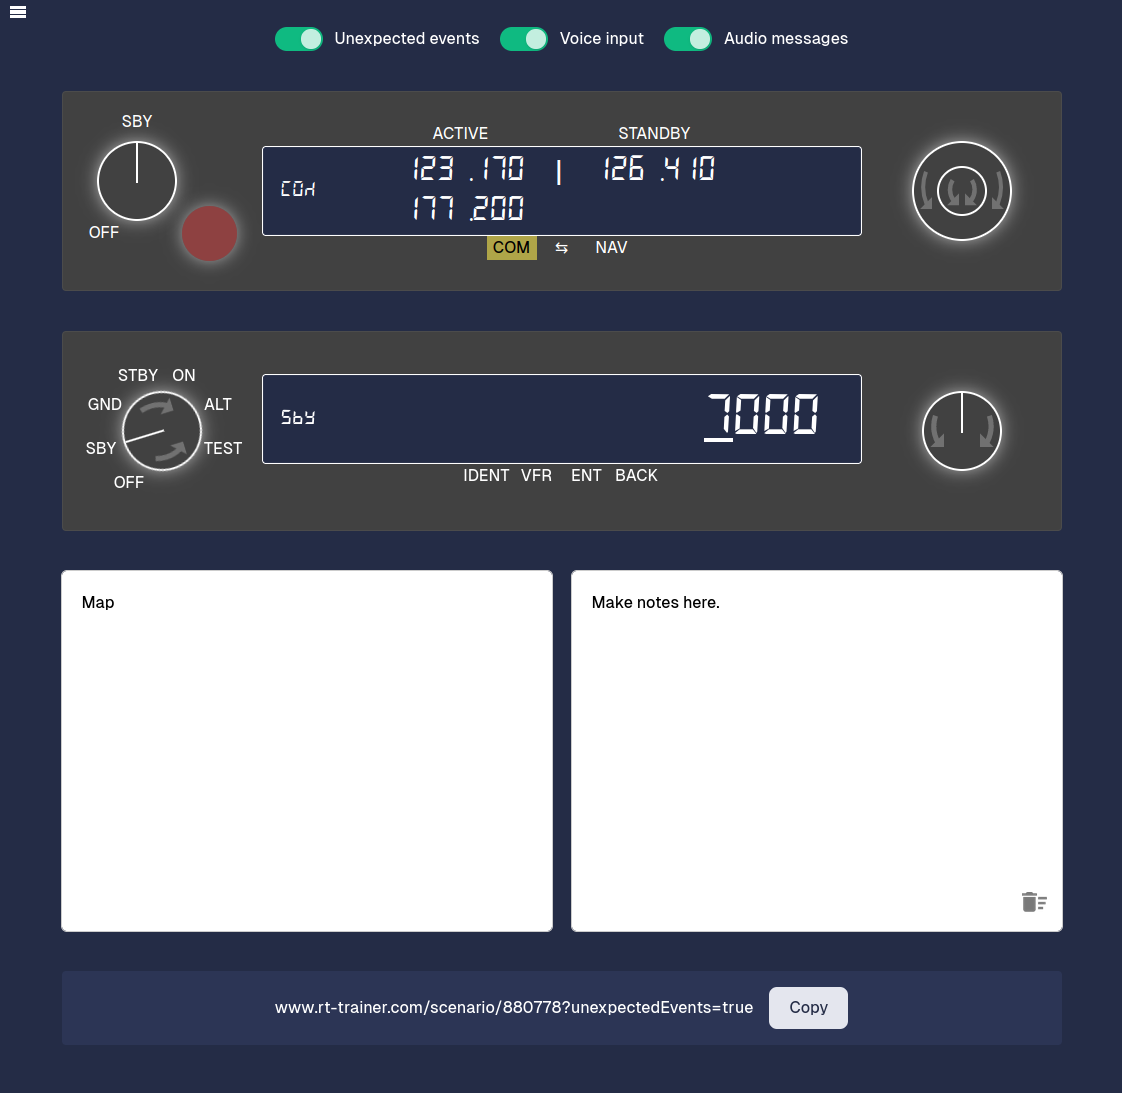
\includegraphics[scale = 0.47]{../document-resources/images/Project-Initial-UI.png}
    \label{initialui}
    \caption{Initial UI design.}
\end{figure}

Given that the system's users are expected to mostly be trainee pilots, the interface has not been designed in an accessible manner in respect to the ARIA web accessibility specification \cite{ARIA}. This manifests in a poor experience for users using non cursor or touchscreen based inputs due to the creative use of certain HTML elements required to implement the interface with only HTML, CSS and JavaScript.

\subsubsection{Next Additions}
Currently the UI visually provides the required functionality of a radio/transponder set that a student might interact with during their R/T exam. The next stage of the UI is to make use of the exposed variables and functions of the UI elements to simulate an exam route and radio calls. This will only be possible once it can communicate with the functioning R/T web server.

Voice input is also not yet implemented, but this is planned to be handled by the browser. Modern browsers implement either their own JavaScript SpeechRecognition class or use the one implemented in WebKit \cite{MDNWebSpeech}, the open source browser engine which powers Safari \cite{WebKit}. After defining the grammar (set of words accepted by the speech recognition), the text generated can be sent to the R/T server in the same way that a text input would be. Similarly the browser implementation of text to speech could be used to read the ATC and other aircraft radio calls to the user.

\subsection{The R/T Web server}
The main challenge of this project, and the main focus for the remainder of the term is the R/T web server, which processes the users' radio calls and generates ATC radio calls in response.

\subsubsection{Design Choices}
The specification document did not mention use of a separate web server for generating R/T. However, it became clear while the front-end was being developed that JavaScript could not perform the complex string operations required for message parsing while being stable. Although Typescript remedies some of JavaScript's inherent unsafe code issues, spotting and handling every other unsafe operation would hinder project progress. Thus the choice was made to write the R/T web server in Rust for its type safety guarantees \cite{Rust}. Rust is a memory safe systems programming language which provides high level syntax with speed comparable to C. The Axum library \cite{Axum} provides the required functionality to serve CRUD (Create, Read, Update, Delete) requests, and is used to handle the web server's endpoints, allowing the majority of the work to be focused on the parsing of radio calls.

\subsubsection{Scenario Generation}
A scenario can be broken down into states, for example in one state the aircraft may be requesting landing clearance at a specified aerodrome. These function as snapshots of the generated flight, which will not be in real time, but instead just a series of states, reflecting the structure of the R/T exam. The states of a scenario are determined entirely by the scenario seed. Currently scenarios are partially hard coded, or lack options for the generation system to choose from. However, the overall process of using the scenario seed to get a large number of unique scenarios from a set of options has been worked out. For example, if the seed is even the route will start at a large airport and end at a small aerodrome, or vice versa for an odd seed. This simple selection system can be extended to more complex decisions, such as aerodrome weather which is based on a simple statistical model determined by a min, average, and max value for each aspect of the weather, sampled by the seed. When the web app determines that the user's state matches the required state sent by the server, it sends the state and R/T call to the server. If the request is valid, the next scenario state is then returned to the web app. The web app state includes the settings of the radio and transponder, in order to simulate setting the correct modes and frequencies.

\subsubsection{Radio call Parsing}
Initially, the use of a Context Free Grammar was considered in order to parse the meaning out of each radio call. Taking inspiration from CS325 Compiler Design \cite{CS325}, an attempt was made to use a similar parser to those found in a compiler. Although R/T is highly standardised, it became apparent that each R/T message is heavily reliant on the previous, thus treating it as context free would not be a suitable abstraction for the process of parsing. Instead of ignoring context, a simpler and easy to implement solution involves the examination of the context alongside the radio call. A simple model of the parsing system is as a Finite Automata. Based on the current scenario state, the scenario seed and the (correctness of the) radio message, the next scenario state can be calculated - alongside an accompanying ATC radio response (in the case a response is expected). This structure makes the R/T web server itself stateless, meaning that it does not hold the current state of any user scenario, instead requires the state to be included in message inputs in order to calculate a response. This reduces the complexity of the solution and potentially reduces development time as no database or state management system needs to be implemented.

\begin{figure}[H]
    \centering
	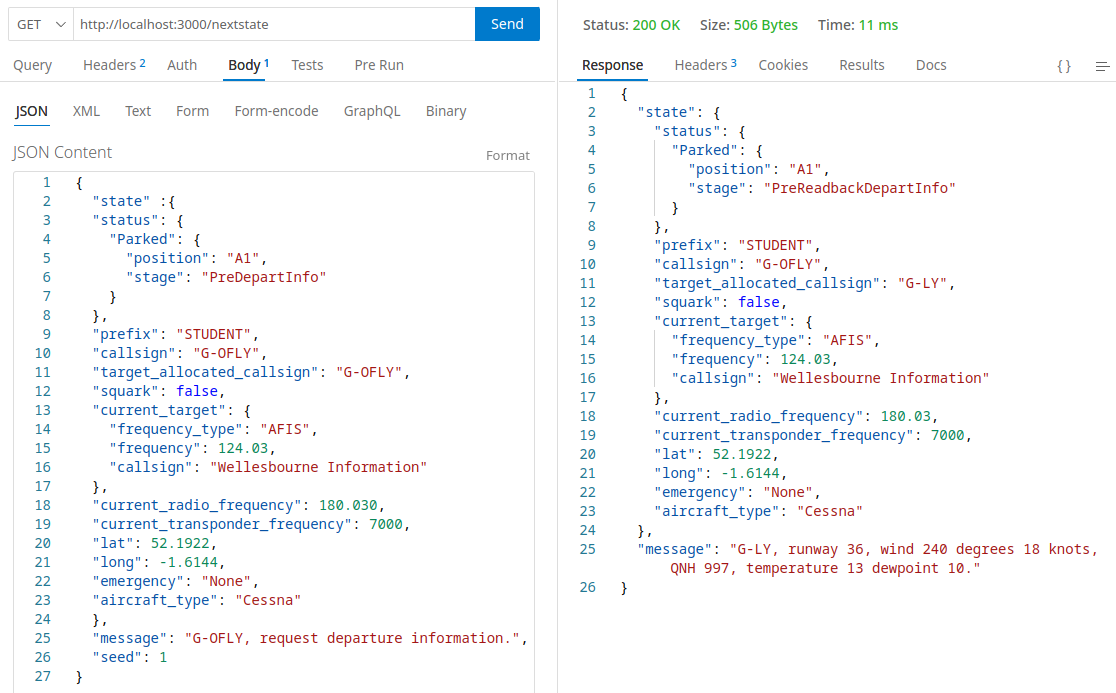
\includegraphics[scale = 0.48]{../document-resources/images/api-screenshot}
    \label{api-endpoint}
    \caption{Content and response of a GET request to the /nextstate endpoint.}
\end{figure}

\subsubsection{Next Additions}
The final part of scenario generation to be planned out is the way point system. Although a large amount of radio calls occur at takeoff and landing, the transiting of airspace in the middle of the flight must be handled too. Way points are points along the flight which important radio calls occur at. For example, if the ATC has requested that the pilot notifies them when they reach a certain position, such a position can be modelled as a way point and the scenario will include the reaching of this way point as a state. One possible approach is to find or create a database of way points. Multiple such databases exist and can be freely accessed via download or API \cite{Google-maps-waypoints, Opennav-database}.